\documentclass{juliacon}
\setcounter{page}{1}

\usepackage{amsmath}

% \usepackage{todonotes}
\usepackage[disable]{todonotes}
\newcommand{\ml}[2][] {\todo[inline,backgroundcolor=orange!20!white, #1]{(ml) #2}}
\newcommand{\bdv}[2][] {\todo[inline,backgroundcolor=blue!20!white, #1]{(bdv) #2}}
\newcommand{\ismail}[2][] {\todo[inline,backgroundcolor=red!20!white, #1]{(ismail) #2}}
\newcommand{\dmitry}[2][] {\todo[inline,backgroundcolor=teal!20!white, #1]{(dmitry) #2}}


\newcommand{\code}[1]{\textsf{#1}}

\begin{document}
% **************GENERATED FILE, DO NOT EDIT**************

\title{ExponentialFamilyManifolds.jl: Representing exponential families as Riemannian manifolds}

\author[1]{Mykola Lukashchuk}
\author[1]{Dmitry Bagaev}
\author[2]{Albert Podusenko}
\author[2]{{\.{I}}smail {\c{S}en\"{o}z}}
\author[1]{Bert de Vries}

\affil[1]{Department of Electrical Engineering, Eindhoven University of Technology, the Netherlands}
\affil[2]{Lazy Dynamics BV, Eindhoven, the Netherlands}


\keywords{Exponential Family, Julia, Manifold Optimization, Optimization, Probability Distributions}

\hypersetup{
pdftitle = {ExponentialFamilyManifolds.jl: Projecting Probability Distributions onto Exponential Family Members},
pdfsubject = {JuliaCon 2024 Proceedings},
pdfauthor = {Mykola Lukashchuk, Dmitry Bagaev},
pdfkeywords = {Probability Distributions, Optimization, Manifold Optimization, Julia, Exponential Family},
}


\maketitle
% \bdv{Please update Overleaf document title to Mykola-2025-JuliaCon-ExponentialFamilyManifolds.}

% \bdv{No email address to contact you?}
% \ml{Yeah, it's strange. I have checked other papers that have been published, and there are no author emails.}

\begin{abstract}
\texttt{ExponentialFamilyManifolds} implements exponential family natural parameter spaces as Riemannian manifolds, enabling geometric optimization over probability distributions. The package automatically manages parameter constraints, such as ensuring the positive definiteness of normal distribution covariance matrices, while providing advanced optimization techniques through the integration of \texttt{ExponentialFamily} with \texttt{Manifolds}. Applications for maximum likelihood estimation and variational inference demonstrate the package's practical utility.
% Optimization over probability distributions is central to many probabilistic inference tasks. While the exponential family parameterization makes such problems tractable, their natural parameter spaces often lack Euclidean structure, complicating standard optimization methods. ExponentialFamilyManifolds.jl addresses this by implementing these parameter spaces as Riemannian manifolds. By bridging ExponentialFamily.jl and Manifolds.jl, the package enables geometric optimization techniques like natural gradient descent while ensuring updates remain in valid parameter regions. We demonstrate the package's utility in maximum likelihood estimation and variational inference tasks, showing how it seamlessly integrates geometric optimization into Julia's probabilistic modeling ecosystem.
\end{abstract}

% \keywords{}
% \bdv{Always put keywords in alphabetical order.}
\section{Introduction}

Probabilistic inference problems can often be formulated as optimization problems, such as maximum likelihood estimation (MLE) or variational inference (VI) \cite{blei_variational_2017}. In practice, this often involves optimizing over a space of probability distributions to find one that best fits the data (MLE) or approximates a target distribution (VI). Unfortunately, direct optimization over arbitrary probability distributions is intractable. To address these challenges, we often resort to solutions within parametric families, with the exponential family of distributions being a popular choice. This family includes many common distributions, such as Gaussian, Dirichlet, and Wishart distributions. Any member of this family can be written as
\begin{equation*}\label{eq:exponential-family}
p(x|\eta) = h(x)\exp\left(\eta^\top T(x) - A(\eta)\right),
\end{equation*}
where $\eta$ are the natural parameters. Although this parametrization makes optimization more tractable, challenges remain due to the geometric constraints on the parameter space. For example, the covariance matrices of a Normal distribution must be positive definite.

We present \texttt{ExponentialFamilyManifolds}, a Julia \cite{bezanson2017julia} package that addresses these challenges by implementing the parameter spaces as Riemannian manifolds. By bridging \texttt{ExponentialFamily} \cite{Senoz_ExponentialFamily_jl_2023} and \texttt{Manifolds} \cite{axen_manifoldsjl_2023}, the new package enables geometrically-aware optimization techniques to handle parameter constraints automatically using \texttt{Manopt} \cite{bergmann_manoptjl_2022}.

\section{A tour through \texttt{ExponentialFamilyManifolds}}
In this section, we introduce the \code{NaturalParametersManifold} interface, the core functionality of our package. We then demonstrate how this interface can be applied to optimization tasks such as maximum likelihood estimation and variational inference.

\subsection{The core interface: \code{NaturalParametersManifold}}
% \dmitry{What \textit{types}? There aren't different "types" of distributions. Here you use programming language jargon to explain a simple idea. Maybe say instead "The \texttt{NaturalParametersManifold} defines a generic interface to work with natural parameters space of an arbitrary distribution from the exponential family."}

The \code{NaturalParametersManifold} defines a generic interface to construct and work with the natural parameters space of an arbitrary distribution from the exponential family. For example, the natural parameters of the Beta distribution form the manifold
\[
\mathcal{M}_{\mathrm{Beta}} \;=\; (-1,\infty) \times (-1,\infty)\,,
\]
which, through \texttt{Manifolds}, can be represented as follows 
\begin{lstlisting}[language=Julia]
ProductManifold(
    ShiftedPositiveNumbers(static(-1)),
    ShiftedPositiveNumbers(static(-1))
)
\end{lstlisting} \texttt{ExponentialFamilyManifolds} provides the following method \begin{lstlisting}[language=Julia]
M = get_natural_manifold(Beta, ())
\end{lstlisting} to construct this manifold. Here, \texttt{M} is the manifold corresponding  to 
\(\mathcal{M}_{\mathrm{Beta}}\,.\)
% \bdv{There is no \texttt{M} in the Listing.} 
Once \texttt{M} is obtained, one can sample a vector of natural parameters on \texttt{M} 
and convert points from it to an instance of \code{ExponentialFamilyDistribution}, 
the main interface in \texttt{ExponentialFamily}. The interface provides a programmatic way to construct and manipulate these manifolds. We highlight the \code{retract} method in the \code{NaturalParametersManifold} interface 
because gradient-based optimization requires a mechanism to move in a given direction (a tangent vector) without leaving the manifold. 
For instance, to move from a point \(\eta\) in the direction \code{X} can be implemented in the following way
\begin{lstlisting}[language=Julia]
ζ = retract(M, η, X)
\end{lstlisting}
This step enforces constraints automatically (e.g., \ \(\zeta \in \mathcal{M}_{\mathrm{Beta}}\)),
freeing practitioners from manual checks of validity.
% \dmitry{
% Why do you spend paper space explaining this? How is this interesting to the story? There are other functions other than \texttt{retract}, right? 
% Why do you want to highlight \texttt{retract} specifically or why should I (as a reader) even bother myself with it? Supposedly this paragraph should help me somehow to understand the next paragraphs, but I dont really see if this is used anywhere below. 
% I would simply remove maybe everything which is below "A key operation" or somehow rewrite it. It feels a bit out of the story and some random fact that doesn't help me to understand what are you talking about. 
% At the very least it should be rewritten. E.g. you mention \texttt{X} first as \textit{direction} (without explaining what direction and where) and then you refer to \texttt{X} as being \textit{tangent vector} (again without explaning what is a tangent vector and why it is not a direction anymore).
% }



\subsection{Using \texttt{ExponentialFamilyManifolds} for Optimization} \label{sec:using_efm}

\texttt{ExponentialFamilyManifolds} transforms distribution-approximation tasks 
(e.g., maximum likelihood estimation or variational inference) into manifold-optimization problems, 
allowing users to focus solely on defining an objective function. 
Listing~\ref{lst:generic_opt} demonstrates a generic workflow for performing gradient-based optimization on a manifold \code{M}: 
first, compute the gradient of the objective \code{f} using \texttt{ForwardDiff} \cite{revels_forward-mode_2016}, 
and then execute \code{gradient\_descent} from \texttt{Manopt}. 
The \code{gradient\_descent} function iteratively applies the \code{retract} method to update parameters along the gradient direction.
\begin{lstlisting}[language=Julia, caption={Generic manifold-based optimization}, label={lst:generic_opt}]
function optimize(M, f, η_init)
    g(M, η) = ForwardDiff.gradient(
            η -> f(M, η), η
    )
    return gradient_descent(M, f, g, η_init)
end
\end{lstlisting}
% \dmitry{What is a \textit{solver}?}

To perform MLE and VI, we only need to define their respective objective functions, the negative log-likelihood for MLE, and the Free Energy for VI, and then use the generic \code{optimize} function to carry on the inference. The objective functions for MLE and VI are provided in listings~\ref{lst:mle} and \ref{lst:vi}, respectively (note that to make the listings smaller in place of \code{ExponentialFamilyDistribution}, we write \code{EFD}). Figure~\ref{fig:comparisons} shows the results of both approaches. The upper panel demonstrates how MLE and VI produce different approximations to the same target distribution, while the bottom panel compares different families of the approximating distribution.

\begin{lstlisting}[language=Julia, caption={Objective functions for MLE}, label={lst:mle}]
function f_mle(M, η, samples)
    dist = convert(EFD, M, η)
    return -mean(logpdf(dist, s) for s in samples)
end
\end{lstlisting}

\begin{lstlisting}[language=Julia, caption={Objective functions for VI}, label={lst:vi}]
function f_vi(M, η, t, size)
    q = convert(EFD, M, η)
    samples = rand(MersenneTwister(22), q, size)
    diff(s) = logpdf(t, s) - logpdf(q, s)
    return -mean(diff, samples)
end
\end{lstlisting}

The \code{optimize} (the Listing \ref{lst:generic_opt}) function demonstrates how gradient descent can be implemented using the \code{NaturalParametersManifold} interface. Additionally, it can be easily adapted to use the natural gradient \cite{amari_natural_1998} by incorporating the Fisher information into the gradient computations, as shown in Listing~\ref{lst:natgrad}. This flexibility allows researchers to perform natural MLE or natural VI by simply reusing the objective functions.

\begin{lstlisting}[language=Julia, label={lst:natgrad}, caption={Implementing the natural gradient}]
function natural_gradient(M, η, f)
    q = convert(EFD, M, η)
    F = fisherinformation(q)
    grad = ForwardDiff.gradient(
        x -> f(M, x), η
    )
    return F \ grad
end
\end{lstlisting}

% \dmitry{Reads confusing. What are these \textit{geometric aspects}? Have they been defined?}

% \section{Acknowledgements}

\begin{figure}[tb]
   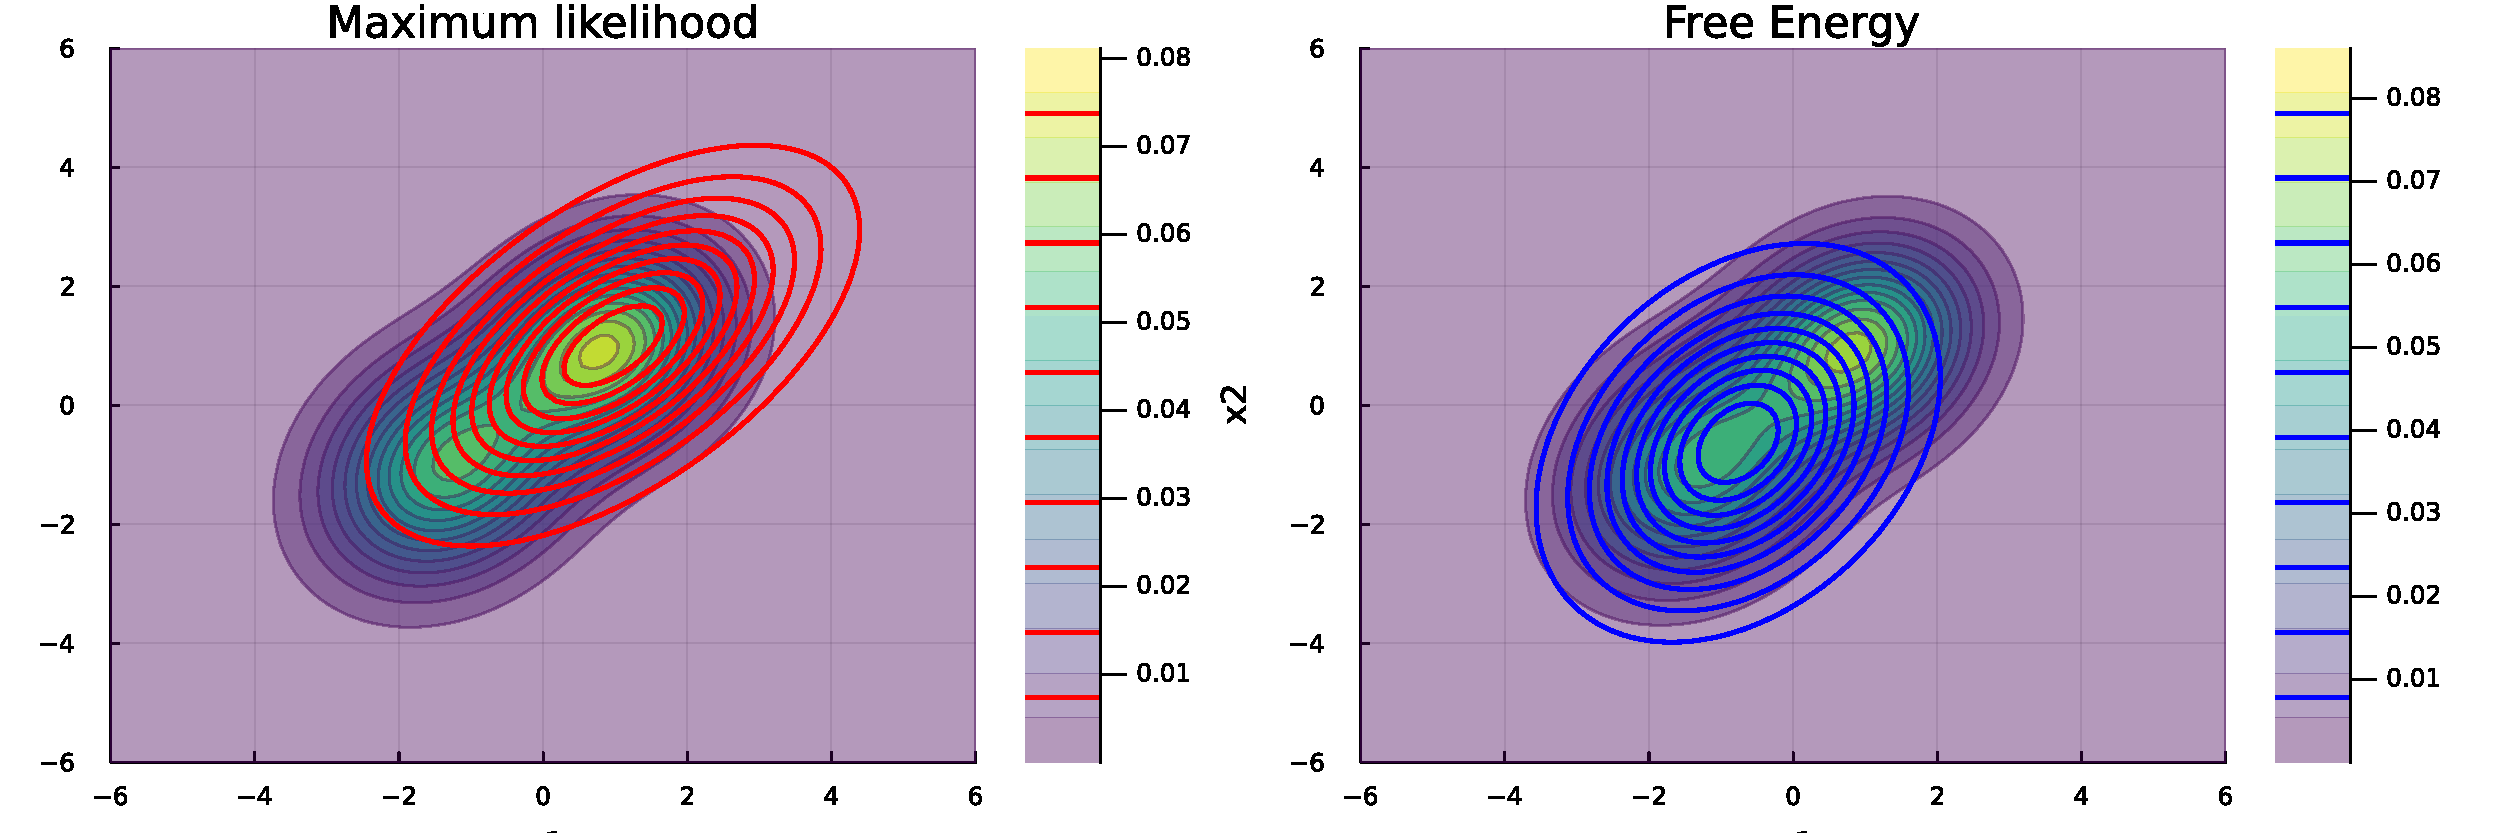
\includegraphics[width=0.48\textwidth]{plots/comparison1.pdf}
   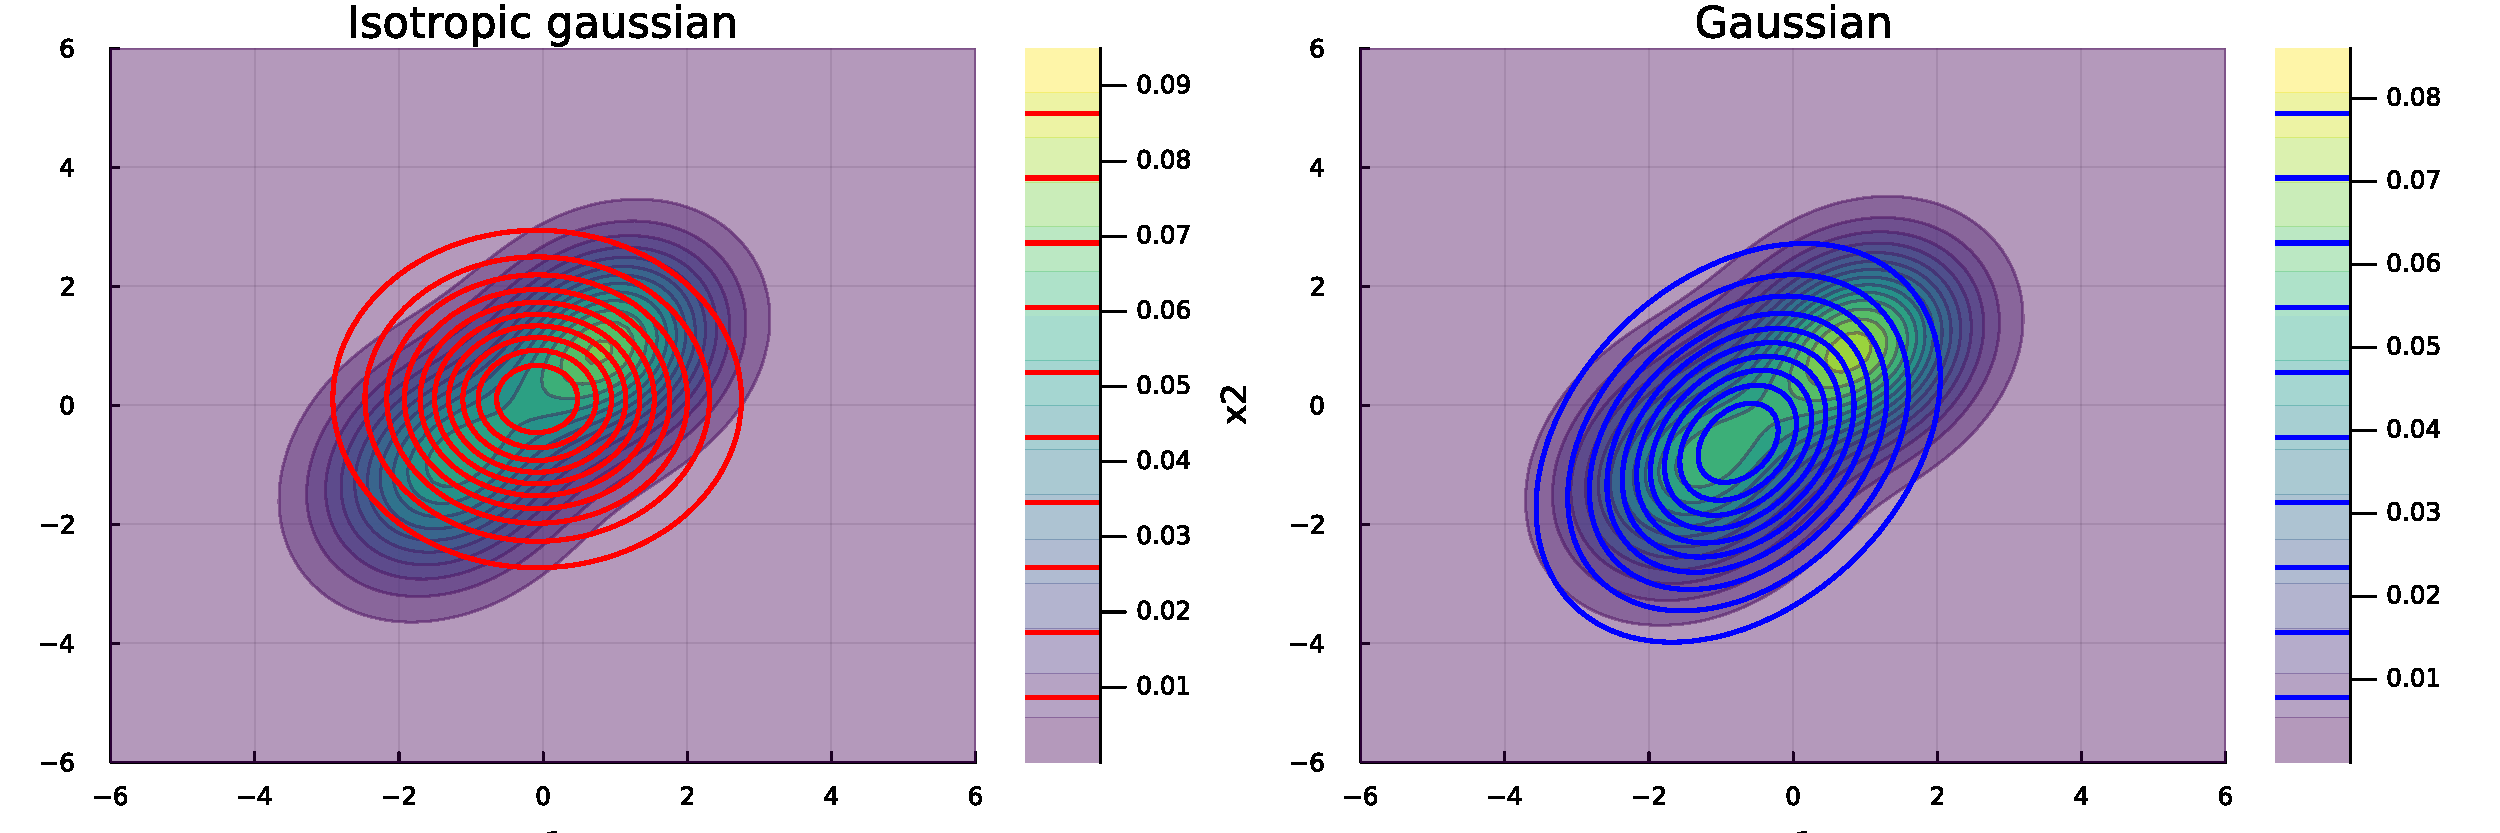
\includegraphics[width=0.48\textwidth]{plots/comparison2.pdf}
   \caption{\textbf{Top:} MLE (red) vs. VI (blue) approximations of a target distribution (shown in the background): a mixture of two Gaussian distributions with different means and covariances. While MLE focuses on covering the target density, VI demonstrates a mode-seeking behavior. \textbf{Bottom:} Isotropic (red) vs.\ full-covariance (blue) Gaussian approximations using the same Free-Energy objective, showing the trade-off between computational efficiency and approximation quality - the isotropic Gaussian requires fewer parameters and converges faster but provides a less flexible fit.}
   \label{fig:comparisons}
\end{figure}

\bdv{Some listings have headers, and some don't. I think you don't need a header when the code fragment is part of a sentence, but if it stands by itself, you need a header. Here, you need a header. Look also at the other Listings.}
\ml{That makes sense, thanks. the only thing I am quite uncomfortable with is how to end the sentence with a code listing; where should I put the period?}
\bdv{Just at the end of the code fragment. Technically, a code fragment inside a sentence should be defined as an single entity by surrounding it by double quotes. Then, you can place the period after the last quotation mark. For brevity, you may deviate from this, but keep it simple. The sentence must flow naturally and be visually easy to read. }

\section{Future work}
While most of the distributions in this package use product manifold geometry, the Fisher-Rao metric~\cite{amari_natural_1998} provides a more suitable geometry for exponential families, potentially leading to more robust optimization (see Listing~\ref{lst:natgrad}). Additionally, extending the package to support mixture families of exponential family distributions could enhance its capabilities since, for example, mixture models can better capture multiple modes in variational inference.

% \dmitry{How do you define "label-switching symmetries" and what is this exactly? Why mixture models help to handle hierarchical models?}

\bibliography{ref}
\bibliographystyle{juliacon}

\end{document}

